\subsection{Cross Talk}

We noticed strage shape of integrated ADC distribution of stopped channel
as the left of figure\ref{cross_talk} shows.
First, we think this is the leak of signal drifted ionization electrons.
However, The shape Monte Carlo Simulation make is very differnt from the shape of DATA.
There we look the signal wave form after FFT cut.
Then, the signal wave form of events which make the mountain
at small integrated ADC is a diffrential of the gaussian shape of stopped channel-1
Figure\ref{cross_talk} shows the signal wave form of stopped channel and stopped channel-1.
This shape is appeared at channel number 1 which cannot enter drifted ionization electron in electric power lines.
From here this bipolar shape is what the voltage change of adjacent channels induced.
This is remarkably looked stopped channel as stopped channel-1 have large intedrated ADC.
We implement this crosstalk phenomenon in Monte Carlo Simulation
by adding bipolar shape of the signal gaussian shape at adjacent channels.
The area of positive region of bipolar shape is 10.5\% of the area of gaussian at adjacent channels.  
The value of 10.5\% is determined by comparing the distribuntion of integrated ADC at stopped channel
between DATA and MC.
The result of comparison of the distribution is shown in section 7.2.

\begin{figure}[htbp]
  \centering
  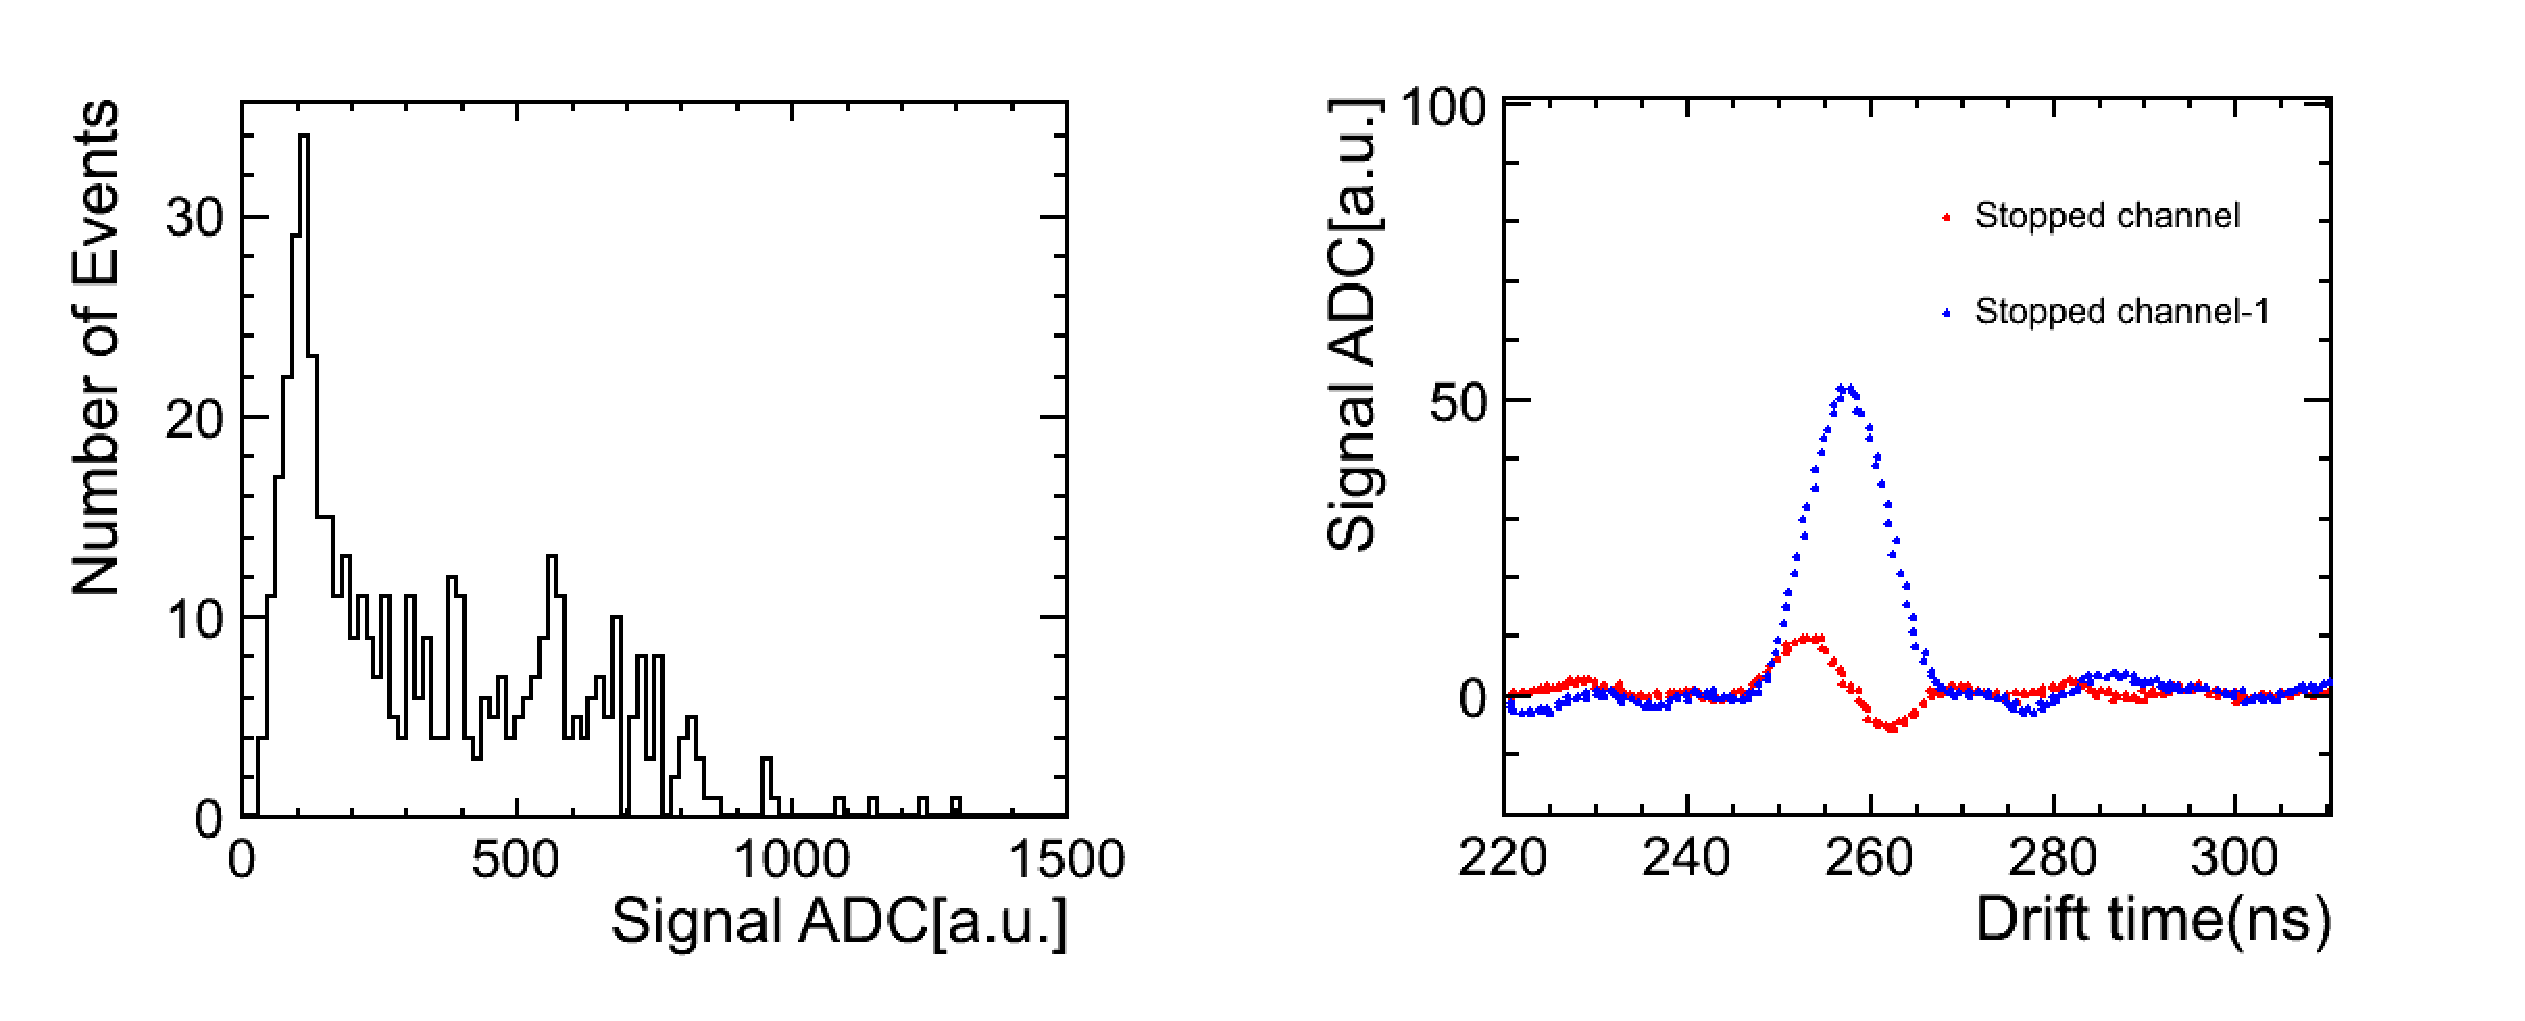
\includegraphics[width=10cm,clip]{fig/cross_talk.eps}
  \caption{Left:Integrated ADC distribution of stopped channel, Right:Signal wave form of stopped channel}
  \label{cross_talk}
\end{figure}

